\documentclass[12pt]{article}
\usepackage[margin=.5in]{geometry}
\usepackage{graphicx}
\usepackage{tikz}
\def\firstcircle{(90:1.75cm) circle (2.5cm)}
\def\secondcircle{(500:1.75cm) circle (2.5cm)}
\title{\vspace*{-3em}HW2}
\author{William Hua}
\date{\today}
\begin{document}
\maketitle
\DeclareGraphicsExtensions{.pdf,.png,.jpg}
%6, 7, 9, 12, 14, 15, 16, 17
%FIXME: make sure to check ALL answers
\section*{6}
\begin{description}
\item[a)] 0, minimum sum is 2
\item[b)] $\frac{4}{36}, (1,4), (4,1), (2, 3), (3, 2)$
\item[c)] $\frac{1}{36}, (6, 6)$
\end{description}

\section*{7}
\begin{description}
\item[a)] No. Since there is a percentage of the voters who are both Independent
    and swing voters, they are not mutually exclusive. 
\item[b)] 
    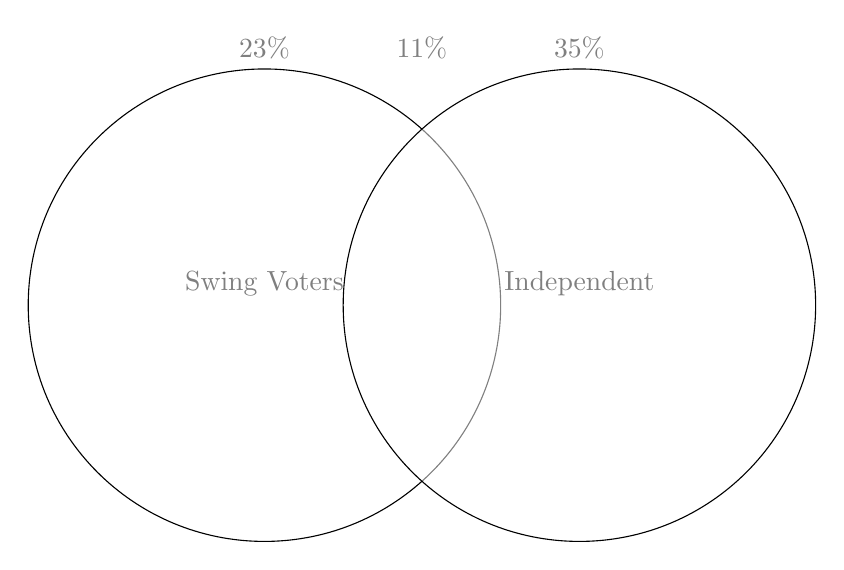
\begin{tikzpicture}
        \begin{scope}[fill opacity=0.5]
            \draw [fill=white, draw=black] (0,0) circle(3) node[text=black, above] {Swing Voters};
            \draw [fill=white, draw=black] (4,0) circle(3) node[text=black, above] {Independent};
            \draw (4, 3) node[text=black, above] {$35\%$};
            \draw (2, 3) node[text=black, above] {$11\%$};
            \draw (0, 3) node[text=black, above] {$23\%$};
        \end{scope}
    \end{tikzpicture}
    %FIXME: draw a venn diagram
\item[c)] $24\%$
\item[d)] $47\%$
\item[e)] $53\%$
\item[f)] They are not independent. $P(Ind \cap Swing) \neq P(Ind)P(Swing)$. 
    $P(Ind \cap Swing) = .11$ and $P(Ind)P(Swing) = .08$
\end{description}

\section*{9}
\begin{description}
\item[a)] Independent
\item[b)] Neither
\item[c)] No
\end{description}

\section*{12}
\begin{description}
\item[a)] $100 - 15 - 28 - 25 = 32\%$
\item[b)] $32 + 25 = 57\%$
\item[c)] $100 - 32 = 68$
\item[d)] I assume that the probability of the two kids missing school are 
    inindependent of each other. $.32 * .32 = .1024$
\item[e)] I make the same assumptions as above. $.68 * .68 = .4624$
\item[f)] Not entirely, since kids usually miss school due to sickness and if 
    one of the kids is sick there is a high chance that the sickness could 
    transfer to the other child.
\end{description}

\section*{14}
\begin{description}
\item[a)] $\frac{15,327}{428,638} = .0357\%$ 
\item[b)] $\frac{141,699 + 44,837}{428,638} = .4351\%$
   \end{description}

\section*{15}
\begin{description}
\item[a)] No, but if it was independent you could.
\item[bi)] $.3*.7=.21$
\item[bii)] $.3 + .7 - .21 = .79$ 
\item[biii)] $\frac{.21}{.7} = .3$
\item[c)] No, $P(A \cap B)$ has to be $.21$ for it to be independent
\item[d)] $\frac{.1}{.7} = .1428$
\end{description}

\section*{16}
$\frac{.78}{.8} = .975$

\section*{17}
\begin{description}
\item[a)] $.6 + .2 - .18 = .62\%$
\item[b)] $\frac{.18}{.2} = .9\%$
\item[c)] $\frac{.11}{.33} = .33\%$
\item[d)] It appears that belief is not independent since if that were true 
    the probability of belief given that one is a liberal democrat should 
    not differ from the probability of belief given that one is a 
    convservative republican. 
\item[e)] $\frac{.06}{.34} = .1764$
\end{description}

\section*{22} 
$\frac{.99*.03}{.99*.03 + .02*.97} = .6048\%$
\section*{23}
$\frac{.997*.259}{.997*.259 + .074*.741} = .8248$
\end{document}
